\subsection{Fonctionnalité 6}
Une fois que le plaideur a défini une date pour son intervention (suite à échange de courriers électroniques avec le contact de l'établissement), il met à jour les informations concernant l'intervention (date, heure, nombre d'élèves, ...). Le demandeur reçoit alors un mail de confirmation l'informant du jour de l'heure et du lieu de l'intervention avec le nom et les coordonnées (adresse électronique, téléphone) du plaideur. Le texte de ce message est à définir et à faire valider par le responsable des plaideurs.
 \\
  La figure \ref{mettreAJourInterventions} présente le diagramme de cas d'utilisation de la mise à jour d'information relative à une intervention. La figure \ref{courrielRecapitulatifIntervention} présente la maquette de l'email récapitulatif des informations concernant l'intervention. 
 
\begin{figure}[H]
	\centering
	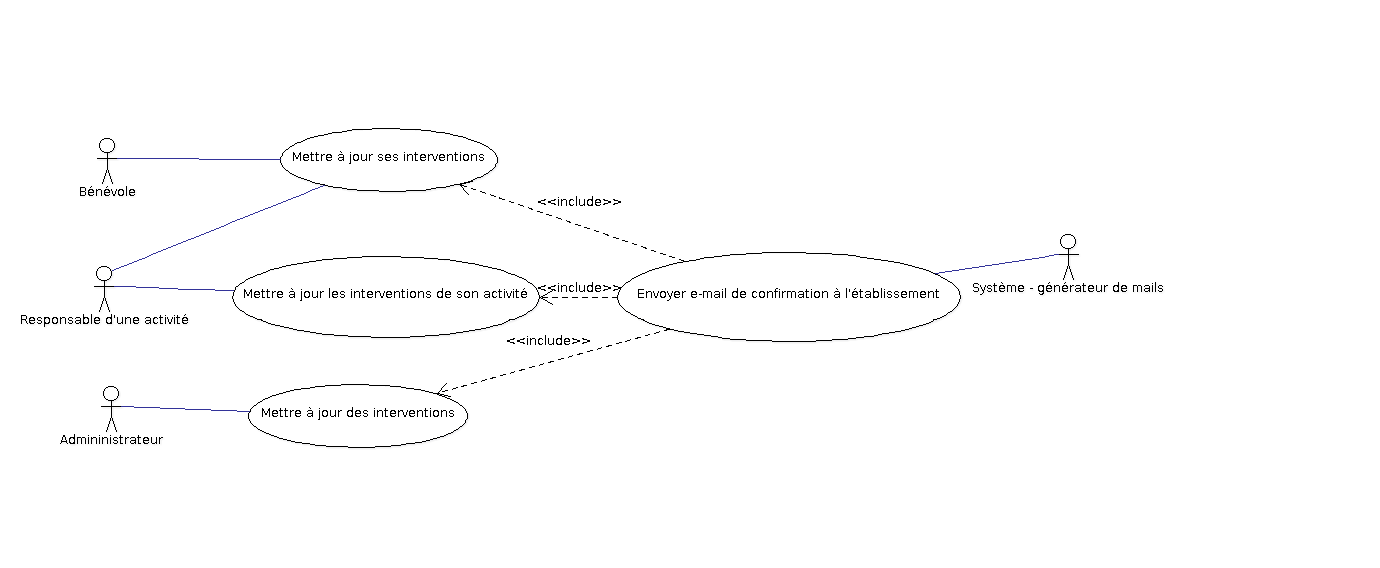
\includegraphics[scale=0.4]{images/casDUtilisation/fonctionnalite6MiseAJourIntervention.png}
	 \caption{Cas d'utilisation~: mettre à jour les informations d'interventions}
	 \label{mettreAJourInterventions}
\end{figure}


% Figure : version 1.00, date 24/02/16, auteur Mélissa Bignoux
\begin{figure}[H]
	\centering
	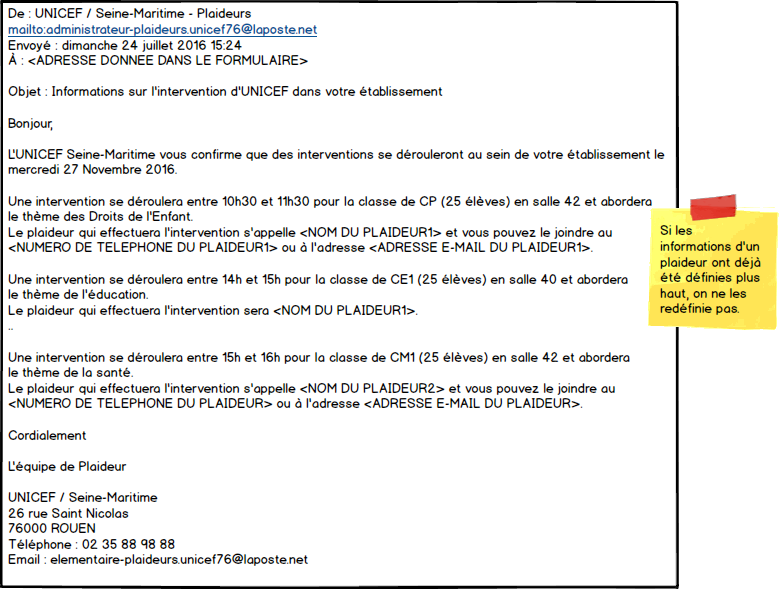
\includegraphics[scale=0.7]{images/maquettes/fonctionnalite6MailDInformationPourLEtablissement.png}
	\caption{Maquette~: Email récapitulatif des informations concernant l'intervention}
	\label{courrielRecapitulatifIntervention}
\end{figure}
